\section{Coordinate Systems}
\label{sec:coordinate}
\graphicspath{{_SISO/Figures/}}

\begin{figure}[!b]
	\centering
		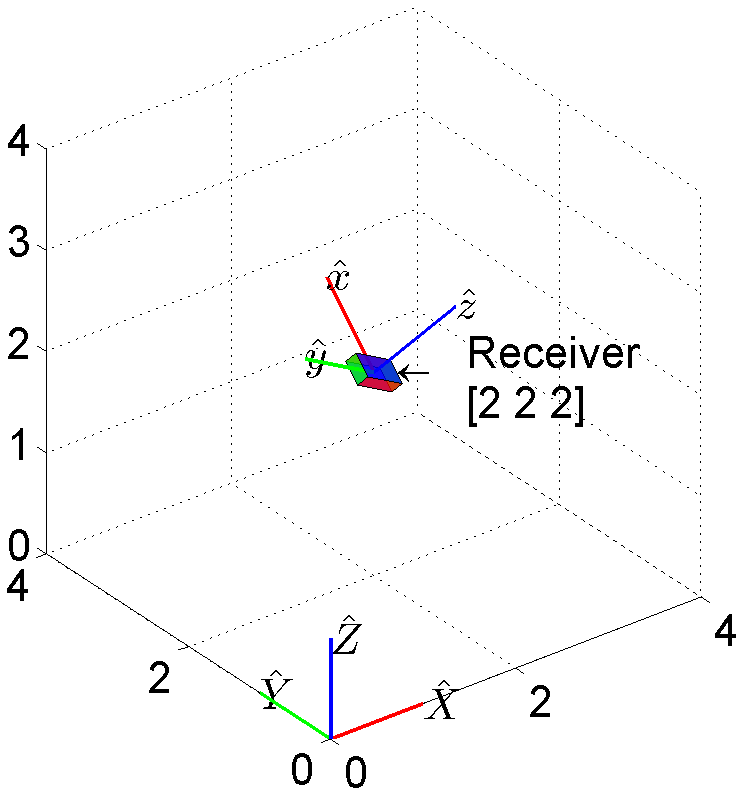
\includegraphics[width=3in]{figRcvrOrientation2.png}
	\caption{Illustration of the coordinate systems used}
	\label{fig:RcvrCoord}
\end{figure}

Establishing a coordinate system convention helps to simplify mathematical representation of distances between different devices and signal propagation path lengths. \figurename{ \ref{fig:RcvrCoord}} illustrates the reference coordinate systems used for all analysis. [$\hat{\bf{X}}$ $\hat{\bf{Y}}$ $\hat{\bf{Z}}$] and [$\hat{\bf{x}}$ $\hat{\bf{y}}$ $\hat{\bf{z}}$] are the basis vectors for the global coordinate system (GCS) and the receiver coordinate system (RCS). A corner of the room in an indoor space is the origin of the GCS while the center of the aperture of the receiver is set as the origin of RCS. The receiver's basis vectors are assumed to always extend parallel to the length, width and surface normal of the sensor. 

Let [$x_{\text{tx}}$ $y_{\text{tx}}$ $z_{\text{tx}}$] be the location of centroid ($C_{\text{tx}}$) of the illumination surface of the transmitter and [$x_{\text{rx}}$ $y_{\text{rx}}$ $z_{\text{rx}}$] be the location of the centroid of the receiver concentrator surface in the GCS. The optical axis is then defined by vector ${\bf{d}}$ as calculated in Eq. \eqref{eqOpAxis} and the vertical distance between the transmitter and receiver is given by ${\bf{d}^{z}}$ as calculated in Eq. \eqref{eqDist}.

\begin{equation}
\label{eqOpAxis}
	{\bf{d}}=\vectthree{x_{\text{tx}}}{y_{\text{tx}}}{z_{\text{tx}}} - \vectthree{x_{\text{rx}}}{y_{\text{rx}}}{z_{\text{rx}}}
\end{equation}

\begin{equation}
\label{eqDist}
	{\bf{d}^{z}}=({\bf{d}}.{\hat{\bf{z}}}){\hat{\bf{z}}}
\end{equation}

